\chapter{Cài đặt và thử nghiệm}
\label{ch:caidat}

\begin{muctieu}
Chương này mô tả môi trường phát triển, cách hiện thực các thành phần chính,
giao diện ứng dụng và chiến lược kiểm thử.
\end{muctieu}

\section{Môi trường triển khai}

Hệ thống được phát triển và thử nghiệm trên máy Windows build 26300 với CPU
Intel Core i5-11400H 2,70~GHz và GPU NVIDIA GeForce RTX~3050 Laptop 4~GB.
Môi trường Python hiện cài PyTorch 2.14.0+cpu nên lần đánh giá trong báo cáo
chạy trên CPU; loader vẫn tự chọn CUDA ở môi trường có bản PyTorch hỗ trợ.
Các thành
phần phần mềm chính đã được liệt kê ở Bảng~\ref{tab:congcu}. Android Emulator
kết nối backend máy chủ qua địa chỉ \code{10.0.2.2:8000}.

Mã nguồn được tổ chức thành hai package chính: \code{backend/} và
\code{mobile/}. Model local, database có dữ liệu tài khoản, dataset, cache và
artifact đánh giá không được commit lên Git. Script setup tải model về đúng
đường dẫn khi môi trường mới chưa có trọng số.

\section{Cài đặt backend}

FastAPI khởi tạo router, mount static media, chạy migration và seed 38 nhãn
trước khi nhận request. Model loader kiểm tra đủ \code{config.json},
\code{preprocessor\_config.json} và trọng số trước khi load local. Nếu thiếu,
script download sử dụng \code{save\_pretrained} để tạo một bản model hoàn
chỉnh. Mã nguồn~\ref{lst:model-loader} minh họa nguyên tắc singleton.

\begin{lstlisting}[language=Python, caption={Nạp model một lần cho toàn bộ tiến trình.}, label={lst:model-loader}]
def get_model_bundle() -> ModelBundle:
    # Load exactly once and reuse the bundle for later requests
    global _bundle
    if _bundle is None:
        with _lock:
            if _bundle is None:
                _bundle = load_model_bundle()
    return _bundle
\end{lstlisting}

Hàm nhận diện giải mã ảnh bằng Pillow, kiểm tra JPEG/PNG và giới hạn pixel,
sau đó dùng processor chính thức của model. Softmax và Top~K được thực hiện
trong \code{torch.inference\_mode}. Tên lớp lấy từ \code{id2label}, không
hard-code thứ tự nhãn.

\section{Cơ sở dữ liệu và catalog công thức}

SQLAlchemy khai báo chín model quan hệ. Alembic quản lý migration ban đầu,
metadata giấy phép và metadata xác minh. Importer đọc hai catalog JSON và
media manifest, kiểm tra schema, URL, nguồn, nguyên liệu, bước nấu, thời gian,
khẩu phần và ảnh trước khi mở transaction. Cập nhật dựa trên slug nên chạy
lại không sinh ID món mới hay làm mất liên kết yêu thích.

Audit hiện xác nhận 38/38 món đã xuất bản, 38 ảnh và metadata đầy đủ. Database
có 348 dòng nguyên liệu, 205 bước và 85 nguồn tham khảo. Ảnh hiển thị được đổi
sang WebP và phục vụ tại \code{/media/dishes}; dataset train không được dùng
làm ảnh giao diện.

\section{Cài đặt ứng dụng Flutter}

Điểm vào là \code{mobile/lib/main.dart}. Các model Dart ánh xạ JSON API;
\code{AppState} quản lý phiên, catalog, yêu thích và lịch sử;
\code{ApiClient} chịu trách nhiệm JSON, refresh token và retry một lần;
\code{AiService} gửi multipart. Token được lưu trong
\code{flutter\_secure\_storage}, còn cache danh mục gần nhất sử dụng shared
preferences.

Luồng camera cho phép chụp hoặc chọn từ thư viện, xem preview và gửi ảnh.
Trong thời gian chờ, thao tác gửi lặp bị khóa. Màn kết quả chỉ hiển thị Top~1,
confidence, nút xem công thức và liên kết phản hồi nhỏ. Nhấn thẻ công thức mở
trực tiếp món trong \code{recognizedDish}, không yêu cầu tìm lại.

\begin{lstlisting}[caption={Ghép URL ảnh tương đối với base URL phía client.}, label={lst:image-url}]
Uri resolveMediaUrl(String value) {
  // Keep absolute URLs; resolve backend media paths centrally
  final parsed = Uri.parse(value);
  if (parsed.hasScheme) return parsed;
  return Uri.parse(ApiConfig.baseUrl).resolve(value);
}
\end{lstlisting}

\section{Giao diện ứng dụng}

Hình~\ref{fig:ui-auth-home} cho thấy màn đăng nhập và trang chủ. Giao diện
dùng xanh lá làm màu thương hiệu, nền kem, điểm nhấn cam và kiểu chữ hỗ trợ
tiếng Việt. Các trạng thái loading, rỗng, lỗi mạng và fallback ảnh được xử
lý riêng.

\begin{figure}[htbp]
\centering
\begin{minipage}[t]{0.31\textwidth}\centering
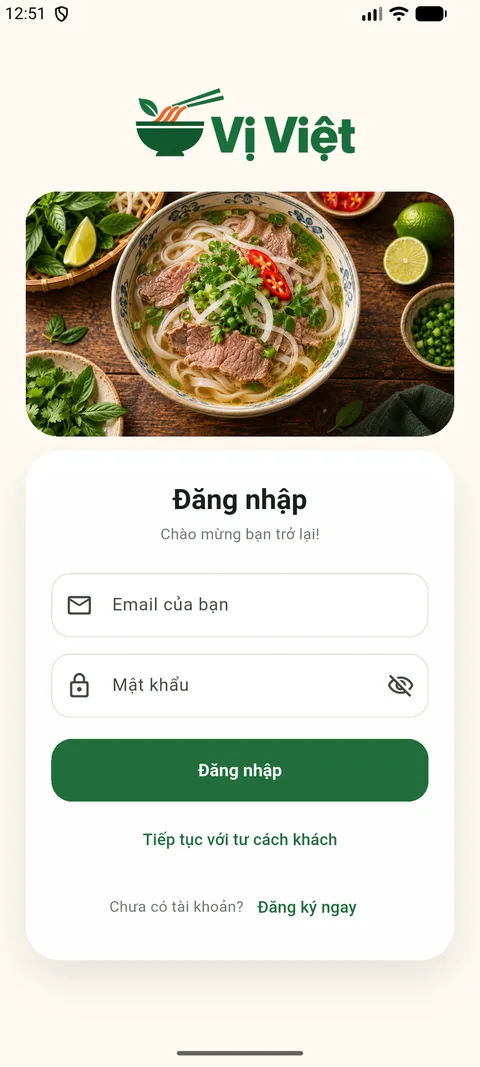
\includegraphics[width=\linewidth,height=.42\textheight,keepaspectratio]{figs/ui/login.png}\\[3pt]
\small Đăng nhập
\end{minipage}\hfill
\begin{minipage}[t]{0.31\textwidth}\centering
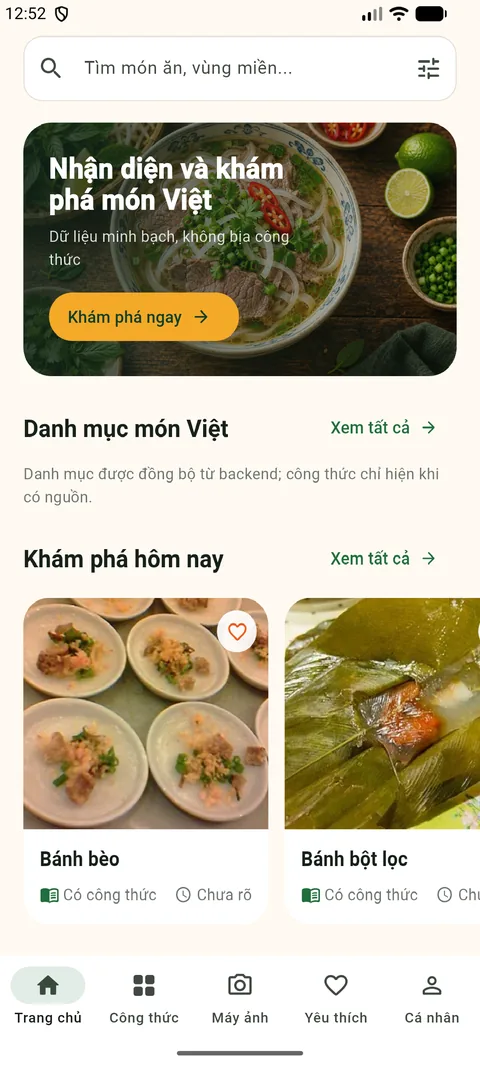
\includegraphics[width=\linewidth,height=.42\textheight,keepaspectratio]{figs/ui/home.png}\\[3pt]
\small Trang chủ
\end{minipage}\hfill
\begin{minipage}[t]{0.31\textwidth}\centering
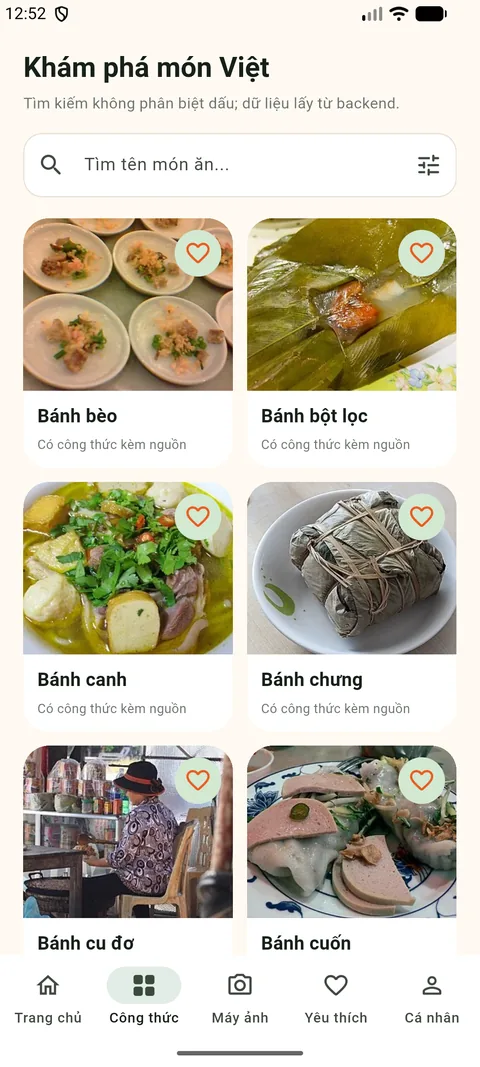
\includegraphics[width=\linewidth,height=.42\textheight,keepaspectratio]{figs/ui/recipes.png}\\[3pt]
\small Danh mục công thức
\end{minipage}
\caption{Các màn hình đăng nhập, trang chủ và danh mục.}
\label{fig:ui-auth-home}
\end{figure}

Hình~\ref{fig:ui-ai-recipe} minh họa luồng nhận diện Phở và khu vực nguồn--bản
quyền. Ảnh kết quả chỉ hiển thị một dự đoán cao nhất theo định hướng tối giản.

\begin{figure}[htbp]
\centering
\begin{minipage}[t]{0.31\textwidth}\centering
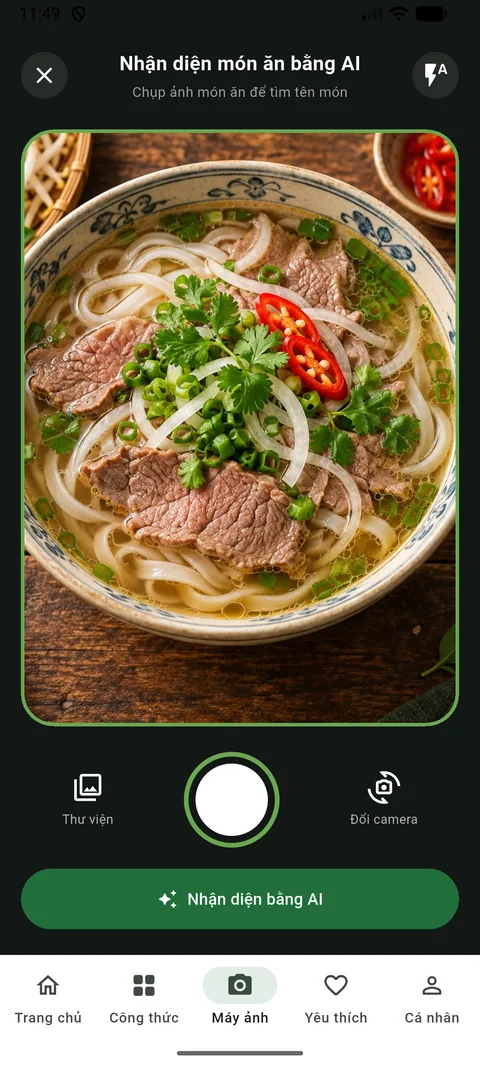
\includegraphics[width=\linewidth,height=.42\textheight,keepaspectratio]{figs/ui/ai-camera-pho.png}\\[3pt]
\small Chọn ảnh Phở
\end{minipage}\hfill
\begin{minipage}[t]{0.31\textwidth}\centering
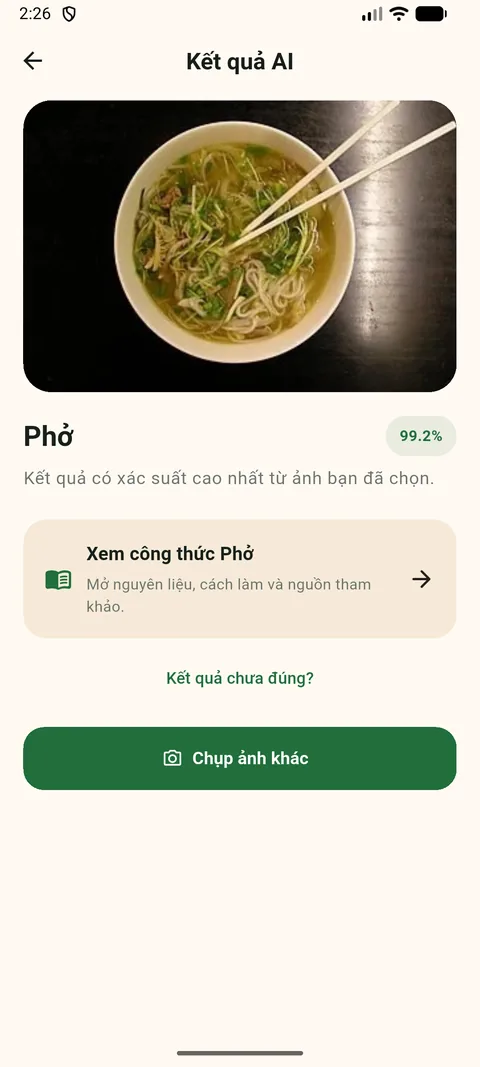
\includegraphics[width=\linewidth,height=.42\textheight,keepaspectratio]{figs/ui/ai-result-pho.png}\\[3pt]
\small Kết quả Top~1
\end{minipage}\hfill
\begin{minipage}[t]{0.31\textwidth}\centering
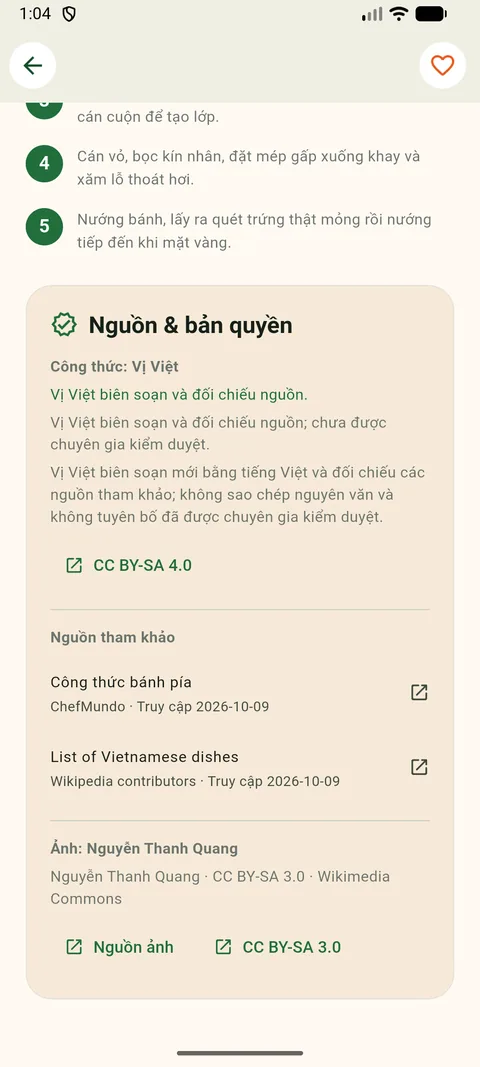
\includegraphics[width=\linewidth,height=.42\textheight,keepaspectratio]{figs/ui/recipe-license.png}\\[3pt]
\small Nguồn và bản quyền
\end{minipage}
\caption{Luồng nhận diện và xem công thức có nguồn.}
\label{fig:ui-ai-recipe}
\end{figure}

\section{Chiến lược kiểm thử}

Backend có 24 test case bao phủ bảo mật, database, model loader, xử lý ảnh,
API và luồng MVP. Flutter có 21 test/widget test cho parse model, refresh
token, optimistic update, màn kết quả, metadata công thức, hồ sơ và điều
hướng đăng ký. Ngoài tự động, audit dữ liệu kiểm tra 38 món, ảnh, metadata và
toàn vẹn catalog. APK debug và hai luồng danh mục--chi tiết, nhận diện--công
thức được dùng để nghiệm thu trên Emulator.

\begin{table}[htbp]
\centering
\caption{Nhóm kiểm thử của hệ thống.}
\label{tab:test-groups}
\begin{tabularx}{\textwidth}{>{\bfseries}p{3.2cm} X}
\toprule
Nhóm & Nội dung \\
\midrule
Backend unit/API & Xác thực, rate limit, ảnh lỗi, CRUD, predict và serializer \\
Flutter & State, parse JSON, điều hướng, dialog, màn kết quả và responsive \\
Data audit & 38 công thức, ảnh, nguồn, thời gian, rollback và idempotency \\
Build & Phân tích tĩnh, test, APK debug và cấu hình Android Studio \\
Emulator & Đăng nhập, tìm kiếm, camera/thư viện, Top~1 và mở công thức \\
\bottomrule
\end{tabularx}
\end{table}
